\documentclass[withoutpreface,bwprint]{cumcmthesis}  %去掉封面与编号页
\usepackage{appendix}
\usepackage{subfigure}	%用于排版多张图片
\usepackage{float}	%用于排版图片位置
\usepackage{pdfpages} % 拼接pdf
\usepackage{url}
\title{\heiti{\zihao{3}身份证号码查验程序设计文档}}

\begin{document}
	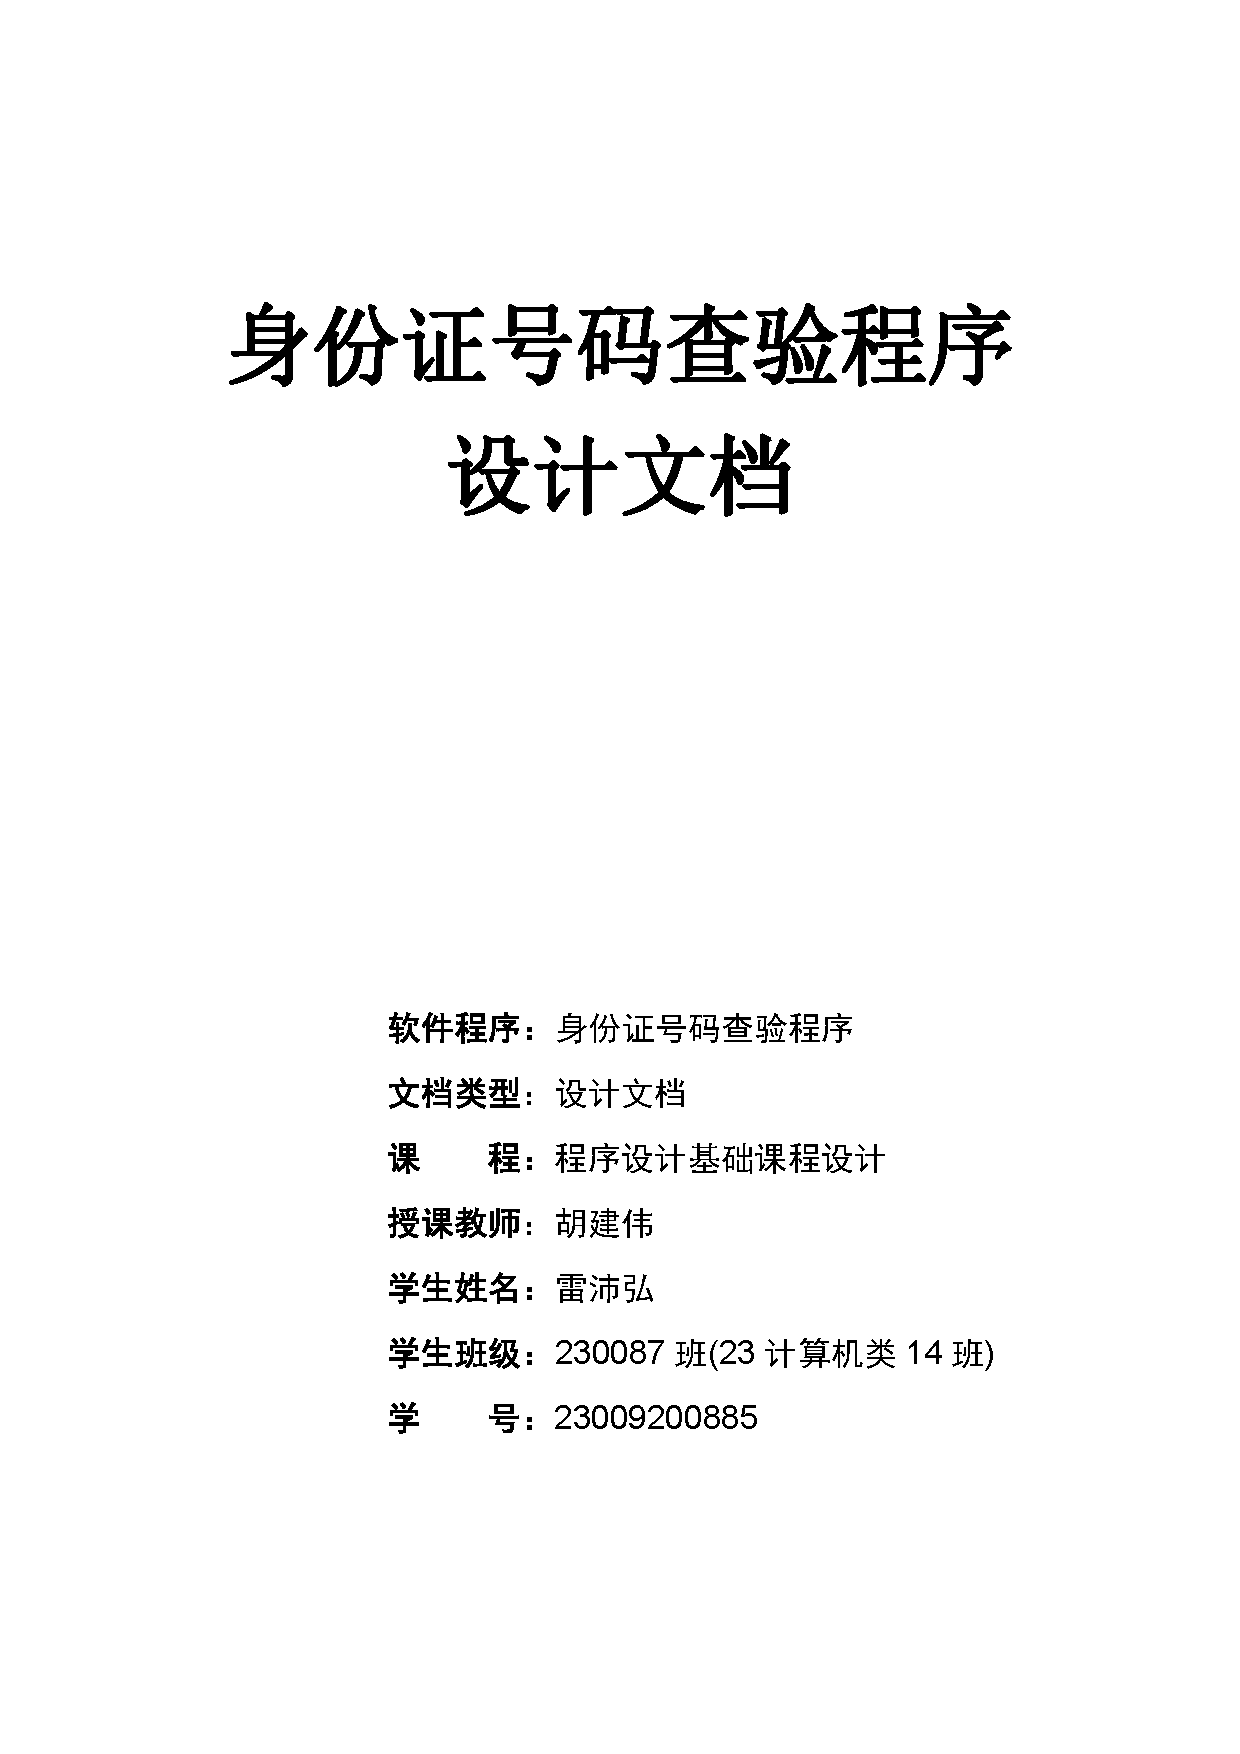
\includepdf{封面1.pdf}
	\tableofcontents
	\maketitle
	
	
	%新的一页
	%\newpage
	%从这里开始是第一个大的标题
	\section{题目解析}%一
	\subsection{需求}
	用户需要通过一个程序查验向该程序输入的身份证号码是否有效。
	\subsection{功能概述} 
	身份证号查验程序将验证输入的所有的身份证号码(一次最多输入10000个,按$Enter$键结束当前身份证号输入,按按q或Q结束所有身份证号输入)是否有效,并对所有无效号码进行提示与输出。
	
	\subsection{查验原理}
	一个合法的身份证号码由17位地区、日期编号和顺序编号加1位校验码组成,共计18位。
	\subsubsection{检验长度}
	程序会先判断输入的身份证号长度是否为18位。如果输入长度不是18位(包括不足或超出18位),程序将提示“身份证号码长度( x位 )不正确,请重新输入”,其中x是检测的当前输入身份证号码的长度,如图(\ref{long})所示。
	
	\begin{figure}[ht]
		\centering
		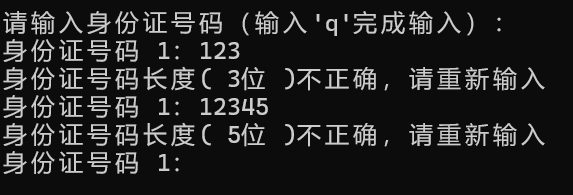
\includegraphics[width=.8\textwidth]{检验长度.png}
		\caption{检测输入身份证号码的长度}
		\label{long}
	\end{figure}
	
	\subsubsection{检验字符}
	在输入的身份证号码长度为18位后,程序将判断号码中是否存在除了0~9和X以外的任何字符。如果存在不合法字符,程序将提醒用户重新输入身份证号,如图(\ref{char})所示。
	
	\begin{figure}[ht]
		\centering
		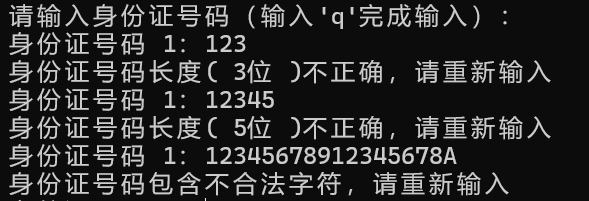
\includegraphics[width=.8\textwidth]{检验字符.png}
		\caption{检测输入身份证号码是否含有非法字符}
		\label{char}
	\end{figure}
	
	\subsubsection{检验校验码}
	在检验完身份证号的长度和字符符合要求后,程序会检验身份证号的校验码是否正确。
	
	
	校验码的计算规则如下:
	\begin{enumerate}
		\item 先对前17位数字加权求和,权重分配为:{7, 9, 10, 5, 8, 4, 2, 1, 6, 3, 
			7, 9, 10, 5, 8, 4, 2};
		\item 然后将计算的和对11取模得到值Z;
		\item 最后按照表(\ref{Z-M})检查值Z有没有对应的校验码M:
		Z:0 1 2 3 4 5 6 7 8 9 10
		M:1 0 X 9 8 7 6 5 4 3 2
	\end{enumerate}
	
	%\vspace{16pt}
	\begin{table}[h] 
		\centering
		\caption{Z值和校验码M值对应关系表} 
		\begin{tabular}{c|ccccccccccc}  
			\toprule  
			Z & 0 & 1 & 2 & 3 & 4 & 5 & 6 & 7 & 8 & 9 & 10 \\  
			\midrule  
			M & 1 & 0 & 9 & 8 & 7 & 6 & 5 & 4 & 3 & 2 & 1  \\  
			\bottomrule  
		\end{tabular}
		\label{Z-M}  
		
	\end{table}  
	
	
	%从这里开始是第二个大标题
	%\newpage
	\section{关键数据结构和功能模块设计}
	
	\subsection{关键数据结构}
	\begin{enumerate}
		\item $char** \quad
		idCards$:动态分配的指针数组,用于存储用户输入的身份证号码,初始化为$NULL$
		\item $int \quad
		numIDCards$:记录已输入的身份证号码数量,初始化为$0$	
		\item $int \quad
		maxIDCards$:设置的最大输入身份证号码数量为$10000$个
		\item $int \quad
		len$:验证当前输入的身份证号码长度,初始化为$0$			
	\end{enumerate}
	
	\subsection{内存处理}
	
	起初,程序将为指针数组动态分配内存,如下所示:
	\begin{lstlisting}[language=c]
		idCards = (char**)malloc(maxIDCards * sizeof(char*));
		if (idCards == NULL) {  // 检验内存是否分配成功
			printf("内存分配失败\n");
			return 1;
		}
	\end{lstlisting}
	
	随后,程序将要求用户逐个输入身份证号码,并通过动态分配内存来存储当前身份证号码:
	\begin{lstlisting}[language=c]
		// 动态分配内存来存储每个身份证号码
		idCards[numIDCards] = (char*)malloc(20 * sizeof(char));  // 身份证号码长度为18位,最后一位为'\0'
		if (idCards[numIDCards] == NULL) {  //  检验内存是否分配成功
			printf("内存分配失败\n");
			return 1;
		}
	\end{lstlisting}	
	
	在内存分配成功后,程序将读取用户输入的身份证号码,去除输入的换行符并检验长度与字符:
	\begin{lstlisting}[language=c]
		// 使用 fgets 安全地读取用户输入的身份证号码
		if (fgets(idCards[numIDCards], 20, stdin) == NULL) {
			printf("读取输入失败\n");
			return 1;
		}
		
		// 去除输入中的换行符
		idCards[numIDCards][strcspn(idCards[numIDCards], "\n")] = '\0';
		len = strlen(idCards[numIDCards]);
		if (idCards[numIDCards][0] == 'q' || idCards[numIDCards][0] == 'Q') {
			break;  // 用户输入 'q' 或 'Q' 结束输入
		}
		if (len != 18) {
			printf("身份证号码长度( %d位 )不正确,请重新输入\n", len);
			//free(idCards[numIDCards]);
			continue;
		}
		for(i=0;i<len;i++){
			if (!(idCards[numIDCards][i] >= '0' && idCards[numIDCards][i] <='9' || idCards[numIDCards][i] == 'X')) {
				printf("身份证号码包含不合法字符,请重新输入\n");
				//free(idCards[numIDCards]);
				break;
			}
		\end{lstlisting}	
		
		数据处理完毕,程序将检验每个身份证号码的校验码是否正确:
		\begin{lstlisting}[language=c]
			// 判断并输出所有无效身份证号码
			for (i = 0; i < numIDCards; i++) {
				if (!validateIDCard(idCards[i])) {
					printf("%s\n", idCards[i]);
				}
			}
		\end{lstlisting}
		
		最终,程序将释放所有动态分配的内存以避免造成内存溢出和泄露。	
		\begin{lstlisting}[language=c]
			// 释放动态分配的内存
			for (i = 0; i < numIDCards; i++) {
				free(idCards[i]);
			}
			free(idCards);
		\end{lstlisting}
		
		\subsection{功能模块设计和程序流程}
		该程序的功能模块流程图如下图所示:
		
		\begin{figure}[H]
			
			\label{chengxuliucheng}     %创立一个标签,下文可以直接引用其中的名字,如图\ref{}所示即可
			\centering
			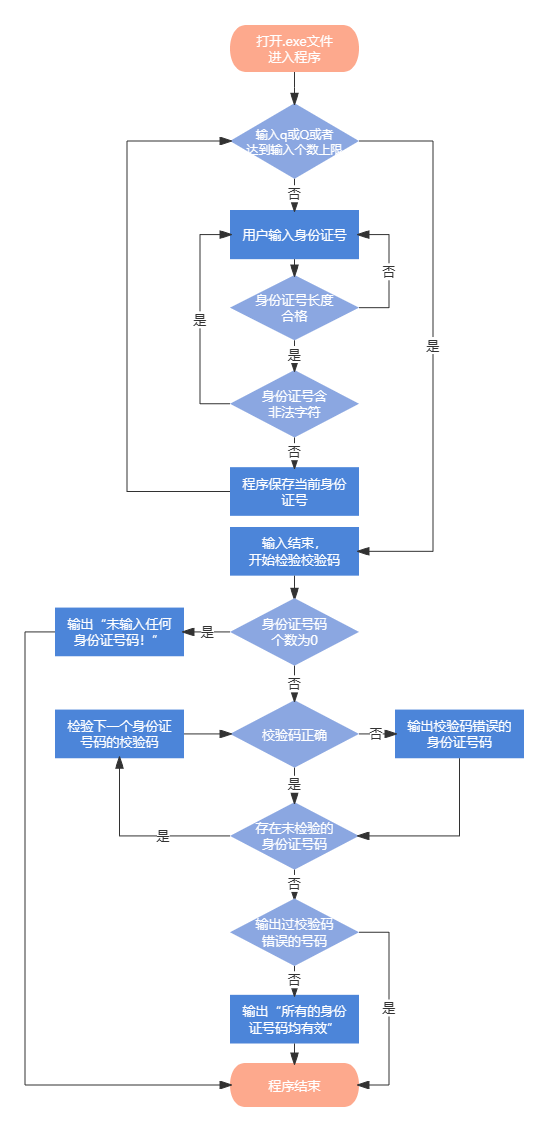
\includegraphics[width=.7\textwidth]{程序流程.png}
			\caption{功能模块设计和程序流程图}  %(引用图片)
		\end{figure}
		
		
		%第三部分开始了
		
		\newpage
		\section {调试与测试}
		\subsection{测试目标}
		\begin{itemize}
			\item 确保身份证号码查验函数 $validateIDCard()$ 能正常运行并返回正确的结果。
			\item 验证程序可以正确读取用户输入的身份证号码。
			\item 确保程序能够正确判断身份证号码的有效性并输出无效的身份证号码。
			\item 验证程序在各种输入情况下的稳定性和鲁棒性。
		\end{itemize}
		
		\subsection {测试方法}
		\subsubsection{测试 $validateIDCard()$ 函数}
		创建多个测试用例,包括合法的身份证号码和非法的身份证号码。
		对每个测试用例,手动计算预期的Z值,并将其与实际结果进行比较以验证函数是否返回了预期的结果。
		确保函数对于各种情况下的边界条件都能正确处理。
		\subsubsection{测试用户输入和内存分配}
		执行程序并按照提示逐个输入身份证号码。
		测试不同情况下的输入,包括合法和非法的身份证号码,长度不正确的输入以及输入 $q$ 或 $Q$ 终止输入等。
		确保程序能够正确读取用户输入的身份证号码,并进行相应的处理。
		通过在程序中设计相应的测试输出以检查内存分配是否成功,以防止内存泄漏或分配失败的情况,比如下面两段代码:
		
		
		\textbf{1)}\textbf{检验是否成功指针数组动态分配内存:}
		\begin{lstlisting}[language=c]
			idCards = (char**)malloc(maxIDCards * sizeof(char*));
			if (idCards == NULL) {  // 检验内存是否分配成功
				printf("内存分配失败\n");
				return 1;
			}
		\end{lstlisting}
		
		\textbf{2)}\textbf{检验是否成功通过动态分配内存来存储当前身份证号码:}
		\begin{lstlisting}[language=c]
			// 动态分配内存来存储每个身份证号码
			idCards[numIDCards] = (char*)malloc(20 * sizeof(char));  // 身份证号码长度为18位,最后一位为'\0'
			if (idCards[numIDCards] == NULL) {  //  检验内存是否分配成功
				printf("内存分配失败\n");
				return 1;
			}
		\end{lstlisting}	
		
		
		\subsubsection{测试身份证号码的有效性判断和输出}  
		输入多个合法和非法的身份证号码。
		确保程序能够正确判断身份证号码的有效性。
		验证程序是否能够正确输出无效的身份证号码。
		
		\subsubsection{测试程序的稳定性和鲁棒性}
		输入大量的身份证号码,包括合法和非法的号码。
		验证程序在处理大量输入时是否仍能正常运行,且不会出现崩溃或异常行为。
		尝试各种边界情况和异常情况,如无输入、输入 $q$ 或 $Q$  终止输入等,确保程序能够正确处理并给出合适的提示。
		
		\subsection{测试记录}
		测试过程记录如下:
		
		先测试能否发现不符合18位长度要求的身份证号码:
		\begin{figure}[ht]
			\centering
			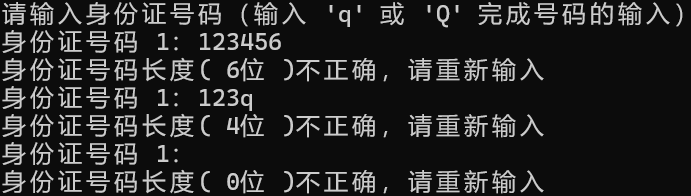
\includegraphics[width=.8\textwidth]{长度.png}
			\caption{检测当前身份证号码长度}
		\end{figure}
		
		在长度符合要求后,测试能否发现含有非法字符的身份证号码:
		\begin{figure}[ht]
			\centering
			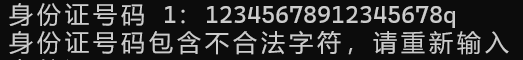
\includegraphics[width=.6\textwidth]{字符.png}
			\caption{检测当前身份证号码是否含有非法字符}
		\end{figure}
		
		如果当前输入的身份证号码的长度和字符均符合要求,则保存该号码。随后,检查输入的身份证号码个数是否达到最大值,如果否,让用户继续输入下一个号码。
		
		\begin{figure}[ht]
			\centering
			
\includegraphics[width=.6\textwidth]{普通号码.png}
			\caption{保存当前号码}
		\end{figure}
		
		\newpage
		检测能否输入 $q$ 或 $Q$ 就能立刻停止输入并开始判断校验码:
		
		\begin{figure}[ht]
			\centering
			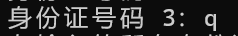
\includegraphics[width=.3\textwidth]{退出.png}
			\caption{检测能否终止输入}
		\end{figure}
		
		最后,检测所有输出的错误身份证号码的校验码是否确实有误。
		以下是测试全程:
		
		\begin{figure}[ht]
			\centering
			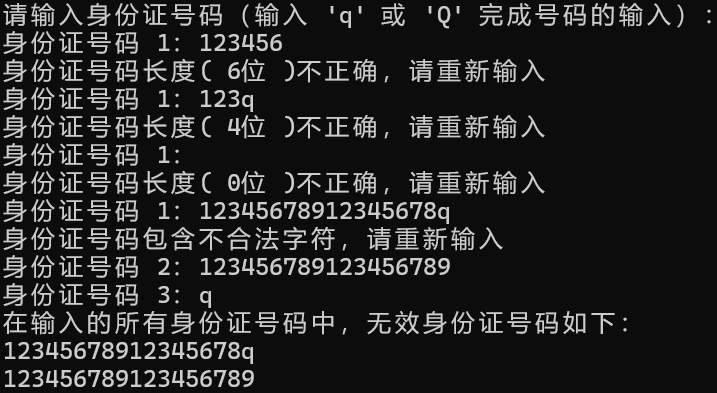
\includegraphics[width=.8\textwidth]{测试全程.png}
			\caption{测试全程}
		\end{figure}
		
		检测输入为空时输出是否为“未输入任何身份证号码!”
		\begin{figure}[ht]
			\centering
			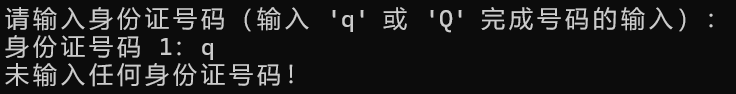
\includegraphics[width=.8\textwidth]{无号码.png}
			\caption{在未输入任何号码时的测试输出}
		\end{figure}
		
		
		内存的分配情况通过断点进行测试:
		\begin{figure}[ht]
			\centering
			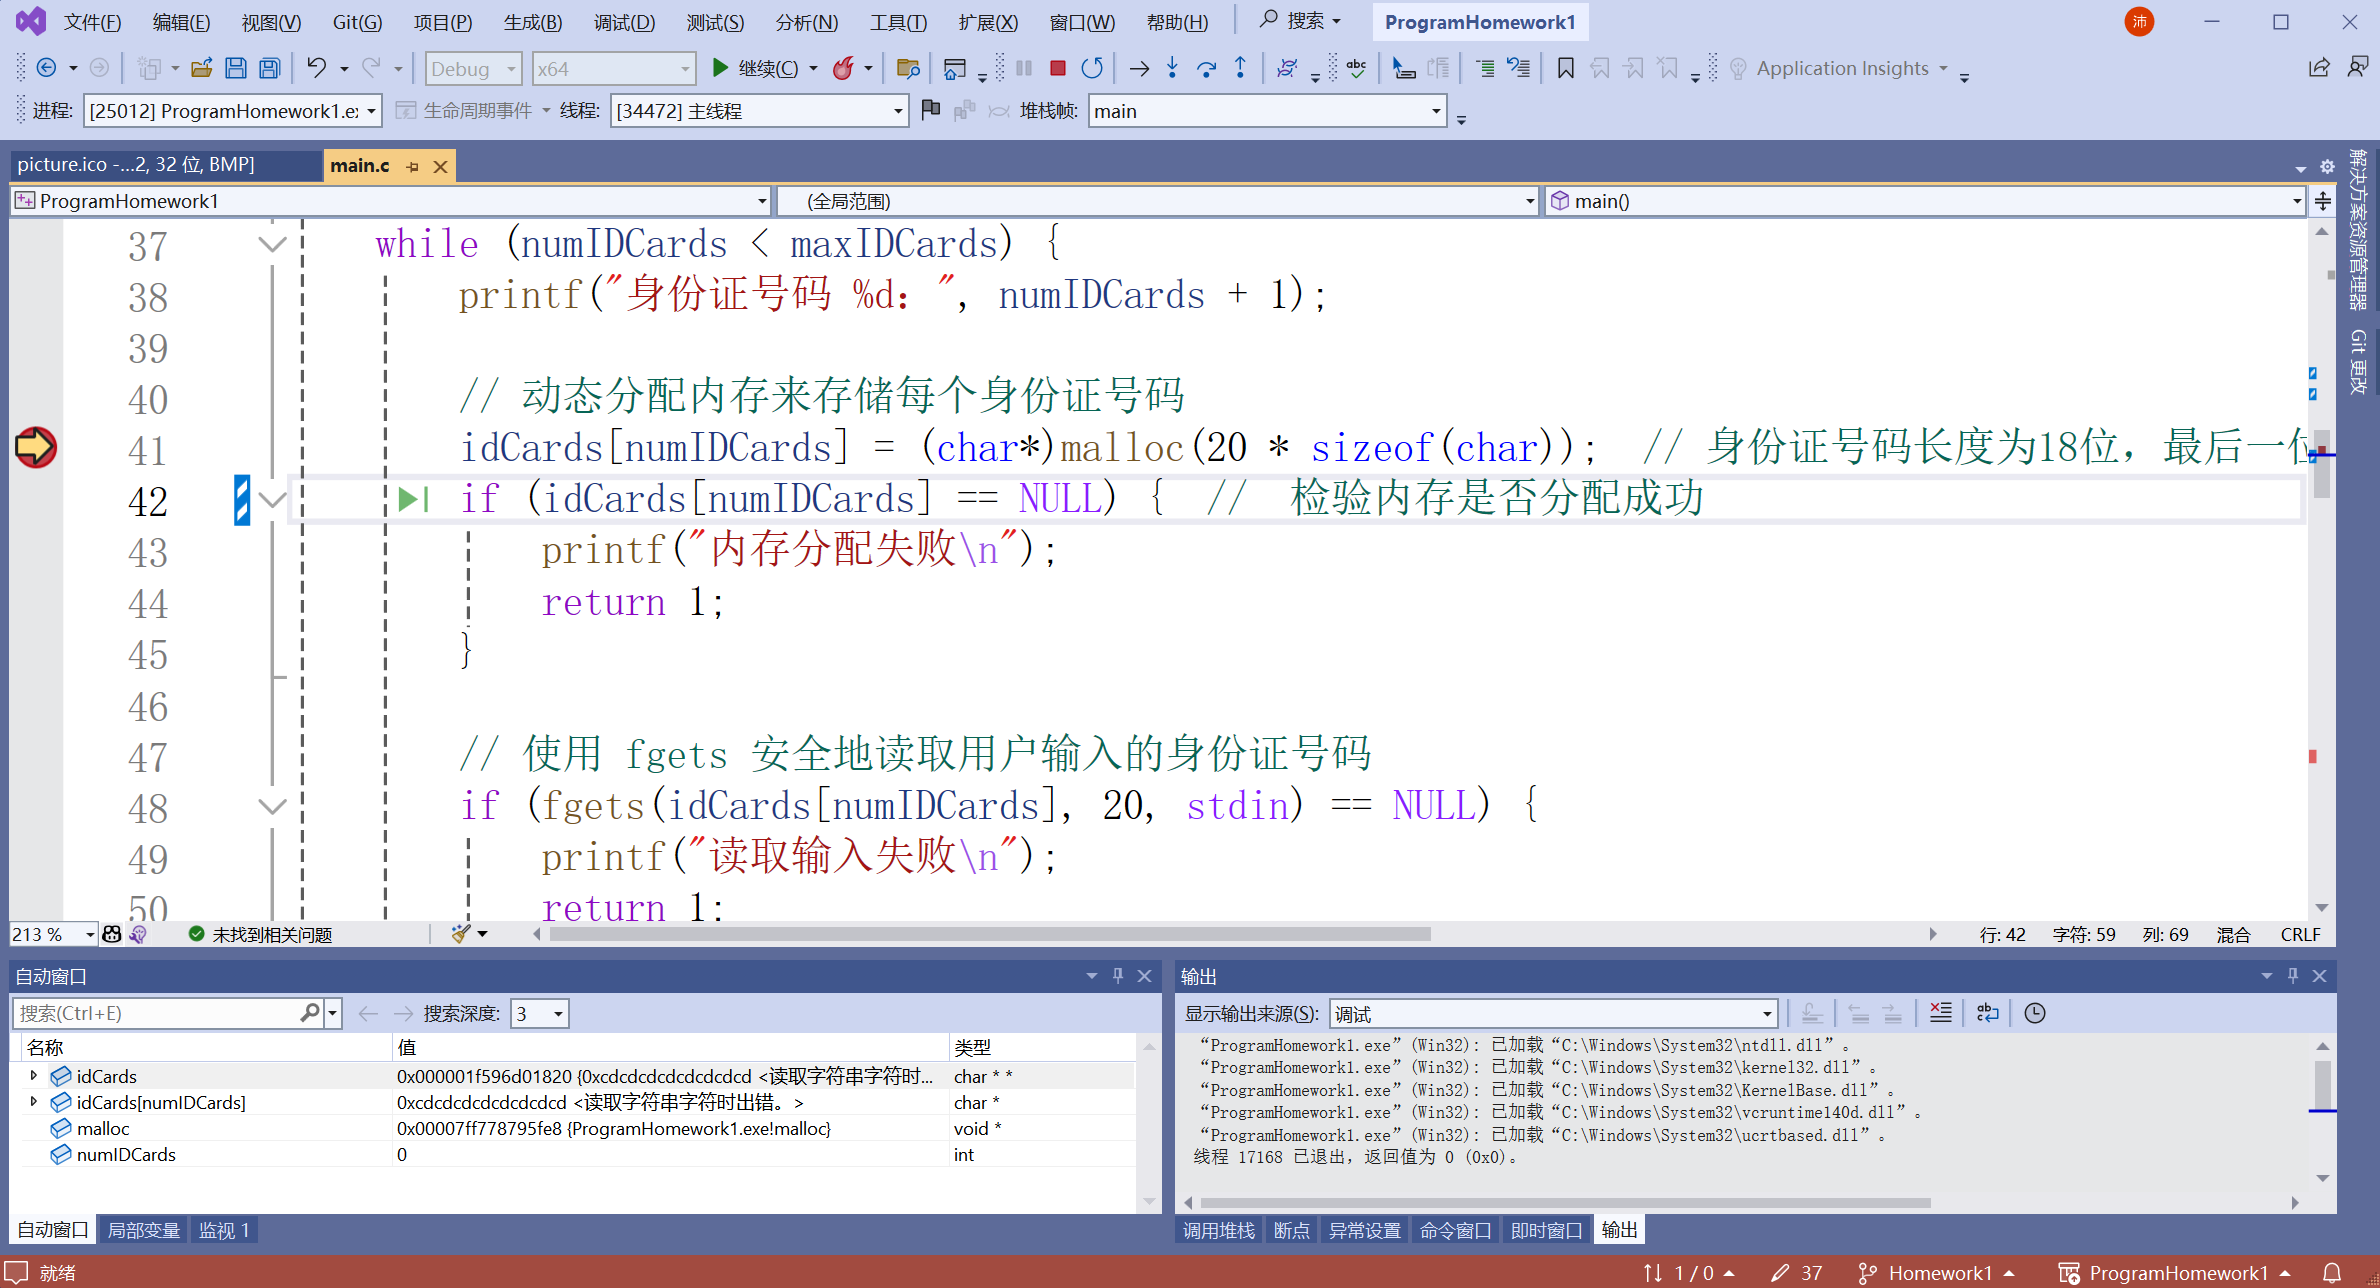
\includegraphics[width=.8\textwidth]{断点1.png}
			\caption{断点测试1}
		\end{figure}
		\begin{figure}[ht]
			\centering
			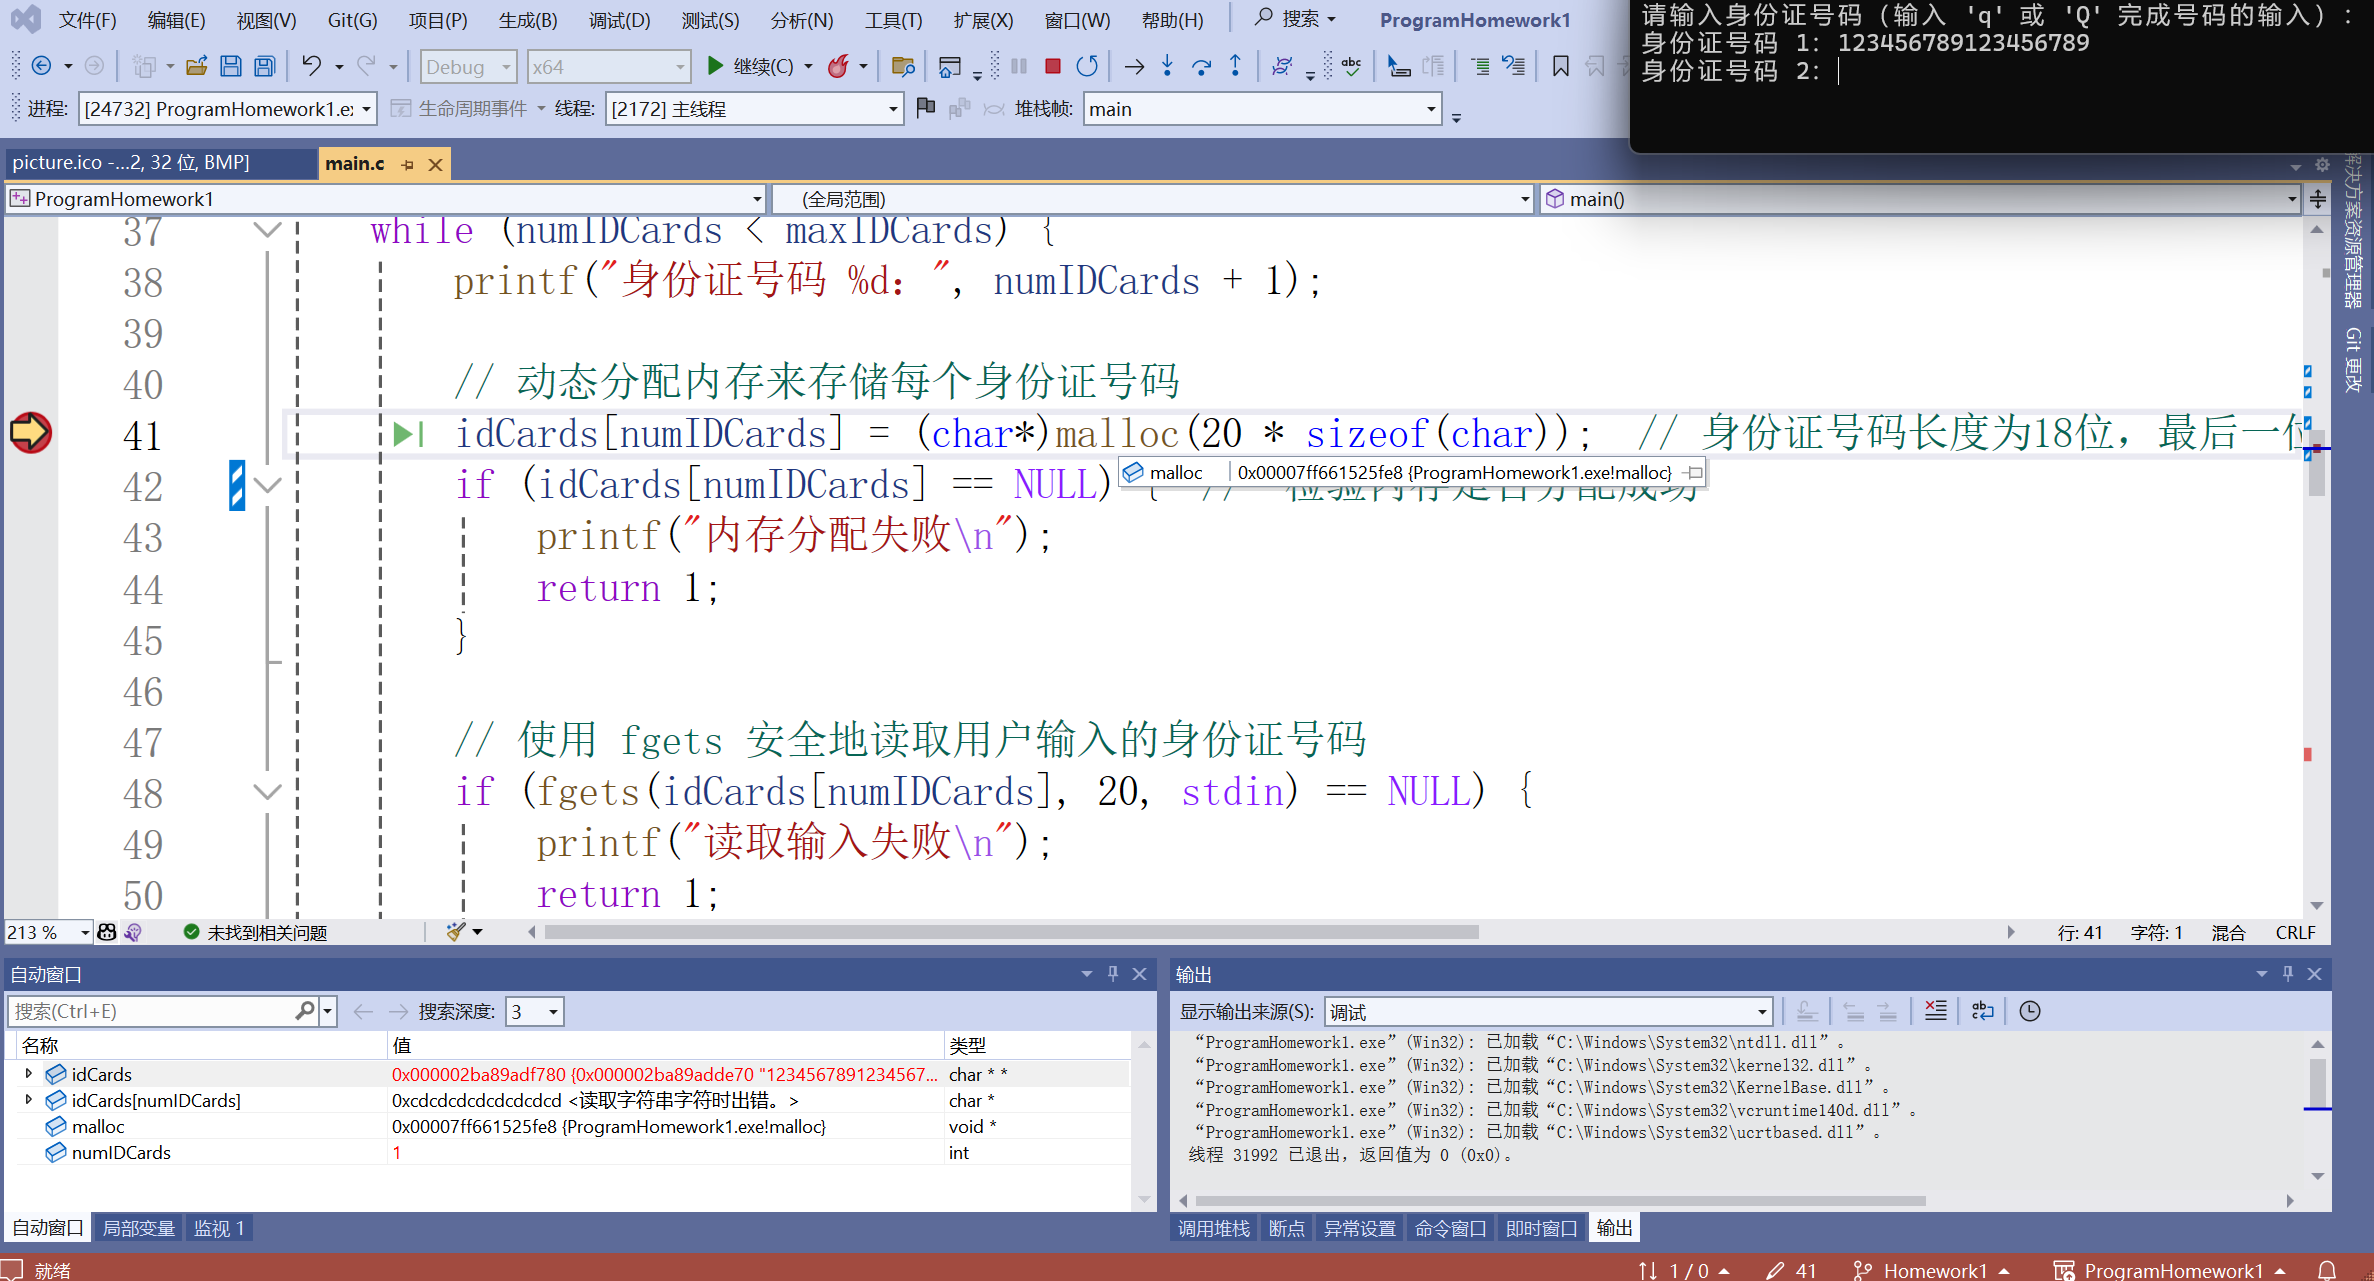
\includegraphics[width=.8\textwidth]{断点2.png}
			\caption{断点测试2}
		\end{figure}
		
		\newpage
		\subsection{测试结果}
		在最终版程序的测试中,所有项目测试结果均符合预期,程序测试通过。
		
		\newpage
		\section{使用程序的注意事项}
		\subsection{程序的使用}
		为了启动该程序,用户需要打开“身份证号查验程序.exe”(如图(\ref{start})所示),之后按照提示操作即可查验用户输入的身份证号是否正确。
		
		\begin{figure}[ht]
			\centering
			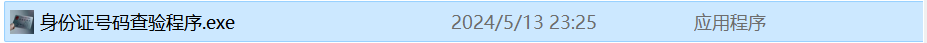
\includegraphics[width=.8\textwidth]{打开程序.png}
			\caption{打开程序}
			\label{start}
		\end{figure}
		
		程序使用完毕后,用户按下回车键即可退出该程序。
		
		\subsection{github仓库}
		该程序的一切源代码(包括本设计文档在内)均可以在
		
		\url{https://github.com/DSCJ1149270594/ProgramHomework} 
		
		的$ Homework1$分支 内下载查看。
		\subsection{更新时间}
		该设计文档和源程序最后更新时间为 2024年5月14日 22:00
		
		\section{程序源代码(C语言)}
		\begin{lstlisting}[language=c]
			#include <stdio.h>
			#include <stdlib.h>
			#include <string.h>
			#include <stdbool.h>
			
			// 查验身份证号码
			int validateIDCard(const char* idCard) {
				int weights[17] = { 7, 9, 10, 5, 8, 4, 2, 1, 6, 3, 7, 9, 10, 5, 8, 4, 2 };  // 对身份证号码前17位数字求加权和的权重
				char checkCodes[11] = { '1', '0', 'X', '9', '8', '7', '6', '5', '4', '3', '2' };  // 校验码M的值
				int sum = 0;
				int i = 0;
				for (i = 0; i < 17; i++) {
					sum += (idCard[i] - '0') * weights[i];  // 计算加权和
				}
				
				int index = sum % 11;  // 取模得到值Z
				char checkCode = checkCodes[index];  // 获取Z对应的校验码M
				
				return (checkCode == idCard[17]);  // 返回校验结果
			}
			
			int main() {
				char** idCards = NULL;  // 用于存储身份证号码的指针数组
				int numIDCards = 0;
				int maxIDCards = 10000;  // 最大输入身份证号码的数量
				int len = 0; // 验证身份证号码长度
				int i = 0;
				// 动态分配内存
				idCards = (char**)malloc(maxIDCards * sizeof(char*));
				if (idCards == NULL) {  //  检验内存是否分配成功
					printf("内存分配失败\n");
					return 1;
				}
				
				// 用户逐个输入身份证号码
				printf("请输入身份证号码(输入 'q' 或 'Q' 完成号码的输入):\n");
				while (numIDCards < maxIDCards) {
					printf("身份证号码 %d:", numIDCards + 1);
					
					// 动态分配内存来存储每个身份证号码
					idCards[numIDCards] = (char*)malloc(20 * sizeof(char));  // 身份证号码长度为18位,最后一位为'\0'
					if (idCards[numIDCards] == NULL) {  //  检验内存是否分配成功
						printf("内存分配失败\n");
						return 1;
					}
					
					// 使用 fgets 安全地读取用户输入的身份证号码
					if (fgets(idCards[numIDCards], 20, stdin) == NULL) {
						printf("读取输入失败\n");
						return 1;
					}
					
					// 去除输入中的换行符
					idCards[numIDCards][strcspn(idCards[numIDCards], "\n")] = '\0';
					len = strlen(idCards[numIDCards]);
					if (idCards[numIDCards][0] == 'q' || idCards[numIDCards][0] == 'Q') {
						break;  // 用户输入 'q' 结束输入
					}
					if (len != 18) {
						printf("身份证号码长度( %d位 )不正确,请重新输入\n", len);
						//free(idCards[numIDCards]);
						continue;
					}
					for(i=0;i<len;i++){
						if (!(idCards[numIDCards][i] >= '0' && idCards[numIDCards][i] <='9' || idCards[numIDCards][i] == 'X')) {
							printf("身份证号码包含不合法字符,请重新输入\n");
							//free(idCards[numIDCards]);
							break;
						}
						
					}
					
					
					numIDCards++;
				}
				if(numIDCards == 0){
					printf("未输入任何身份证号码!\n");
					// 释放动态分配的内存
					for (i = 0; i < numIDCards; i++) {
						free(idCards[i]);
					}
					free(idCards);
					printf("\n请按回车键退出该程序。\n");
					getchar();  // 等待用户按下回车键退出程序
					return 1;
				}
				printf("在输入的所有身份证号码中,");
				_Bool flag = true;
				for (i = 0; i < numIDCards; i++) {
					if (!validateIDCard(idCards[i])) {
						flag = false;
						break;
					}
				}
				if (flag) {
					printf("所有身份证号码均有效。");
				}else {
					printf("无效身份证号码如下:\n");
				}
				
				// 判断并输出所有无效身份证号码
				for (i = 0; i < numIDCards; i++) {
					if (!validateIDCard(idCards[i])) {
						printf("%s\n", idCards[i]);
					}
				}
				
				// 释放动态分配的内存
				for (i = 0; i < numIDCards; i++) {
					free(idCards[i]);
				}
				free(idCards);
				
				printf("\n请按回车键退出该程序。\n");
				getchar();  // 等待用户按下回车键退出程序
				
				return 0;
			}
		\end{lstlisting}
		
	\end{document}